\documentclass{article}
\usepackage{amsmath}
\usepackage{vmargin}
\usepackage{amssymb}
\usepackage{graphicx}
\usepackage{amsfonts}

\title{Boletin Calculo 1}
\author{Manuel Mateo Delgado-Gambino López}
\date{February 2023}

%Settings:
\setpapersize{A4}
\setmargins{2.5cm}       % margen izquierdo
{1.5cm}                        % margen superior
{16.5cm}                      % anchura del texto
{23.42cm}                    % altura del texto
{10pt}                           % altura de los encabezados
{1cm}                           % espacio entre el texto y los encabezados
{0pt}                             % altura del pie de página
{2cm}                           % espacio entre el texto y el pie de página

%Argumentos:
\providecommand{\abs}[1]{\lvert#1\rvert}

\begin{document}

\maketitle

\section{Introduction}
Resolución de ejercicios del Boletín 1, bloque B(1, 2 y 3).
Ejercicio introductivo al temario de la Unidad 1 de Cálculo y a LaTeX.

\section{Pregunta 1}

\setlength{\parindent}{0cm}

Habitualmente, calculamos el límite de una sucesión real $(x_{n})_{n \in \mathbb{N}}$ usando herramientas como el Teorema de Algebra de Límites, los logaritmos o la composición con funciones continuas, evitando el uso de los $\varepsilon$. De todos modos, no conviene perder de vista que siempre que existe el límite de $(x_{n})_{n \in \mathbb{N}}$ podemos hacer igualmente el razonamiento de esa manera. Responde a las siguientes cuestiones para una sucesión real con término general:
$x_{n} = 1 - \frac{1}{\sqrt{n}}$.
    
    \setlength{\parindent}{1cm}
        1.a) Para $\varepsilon = 0.1$, encuentra un índice natural $N_{0,1}$ de tal forma que los términos $x_n$ a partir de ese índice estén a una distancia de $L=1$ menor que dicho $\varepsilon$.

        1.b) Para $\varepsilon = 0.001$, encuentra un índice natural $N_{0,001}$ de tal forma que los términos $x_n$ a partir de ese índice estén a una distancia de $L=1$ menor que dicho $\varepsilon$.

        1.c) Generaliza los anteriores argumentos y encuentra, para cada $\varepsilon > 0$, una fórmula que devuelva un índice natural $N_{\varepsilon}$ de tal forma que los términos $x_n$ a partir de ese índice estén a una distancia de $L=1$ menor que dicho $\varepsilon$.
    

    \subsection{Solución apartado "1.a"}
\begin{equation}
\varepsilon = 0,1 \\
\varepsilon > 0 \text{ y } \exists N_{\varepsilon} \in \mathbb{N} \text{ tal que } n \leq N_{\varepsilon} \\
N_{0,1} < \varepsilon \text{ y } \left| x_{n} - L \right| < \varepsilon
\end{equation}

Calculamos la distancia entre $x_{n}$ y $L$:

\begin{equation}
\left| x_{n} - L \right| < \varepsilon \text{, lo que implica } \left| 1 - \frac{1}{\sqrt{n}} - 1 \right| < \varepsilon \text{, y a su vez } \left| \frac{-1}{\sqrt{n}} \right| < 0,1
\end{equation}

Hemos de hallar un valor $n$ que cumpla:

\begin{equation}
n^{-1} < 0,1 \implies \frac{1}{0,1} < n^{-1} \implies \sqrt{n} > 10
\end{equation}

Solución:

\begin{equation}
n > 100
\end{equation}

Se necesita que $n$ sea mayor que 100 para que se cumpla la siguiente condición:

\begin{equation}
\frac{1}{\sqrt{n}} < 0.1
\end{equation}

$N_{0,1} = 101$ sería la primera solución válida ya que es el primer valor en $\mathbb{N}$ / cumpla la inecuación:

\begin{equation}
\mid x_{n} - 1 \mid < \varepsilon
\end{equation}

    \subsection{Solución apartado "1.b"}
Sea $\varepsilon = 0,001$ y $N_{0,001}$. Considerando la siguiente igualdad:

\begin{equation}
\left| x_{n} - L \right| < \varepsilon
\end{equation}

Y sabiendo que para todo $\varepsilon > 0$, existe $N_{\varepsilon} \in \mathbb{N}$ tal que $n \geq N_{\varepsilon}$, la distancia entre $x_{n}$ y $L$ es menor que $\varepsilon$ si se cumple lo siguiente:

\begin{equation}
\left| 1- \left(\frac{1}{\sqrt{n}} - 1\right) \right| < \varepsilon \implies \left| -\frac{1}{\sqrt{n}} \right| < \varepsilon
\end{equation}

Por tanto, $1/\sqrt{n} < \varepsilon$, lo que implica:

\begin{equation}
\frac{1}{\varepsilon} < \sqrt{n} \implies n > \left(\frac{1}{\varepsilon}\right)^2
\end{equation}

Entonces, para que se cumpla $\left| x_{n} - L \right| < \varepsilon$, se necesita que $n > \left(\frac{1}{\varepsilon}\right)^2 = 10^6$.

\noindent Sabiendo que:
\begin{equation}
\forall \varepsilon > 0, \exists N_{\varepsilon} \in \mathbb{N} \hspace{5mm} / \hspace{5mm} n \geq N_{\varepsilon}
\end{equation}

\noindent La distancia entre $x_{n}$ y $L$ es menor a $\varepsilon$ si se cumple que:
\begin{equation}
| x_{n} - L | < \varepsilon \hspace{5mm} \implies \hspace{5mm} | 1 - \left( \frac{1}{\sqrt{n}} - 1 \right) | < \varepsilon \hspace{5mm} \implies \hspace{5mm} | - \frac{1}{\sqrt{n}} | < \varepsilon
\end{equation}

\noindent Lo que significa que:
\begin{equation}
\frac{1}{\sqrt{n}} < \varepsilon \hspace{5mm} \implies \hspace{5mm} \sqrt{n} > \frac{1}{\varepsilon}
\end{equation}

\noindent Por lo tanto, se concluye que:
\begin{equation}
n > \left( \frac{1}{\varepsilon} \right)^2
\end{equation}

\noindent Y, en este caso específico:
\begin{equation}
n > \left( \frac{1}{0,001} \right)^2 = 1000^2 = 1000001
\end{equation}

\noindent Por lo que, se tiene que:
\begin{equation}
N_{0,001} = 1000001
\end{equation}

\noindent Y para todo $n \geq 1000001$ se cumple que:
\begin{equation}
| x_{n} - L | < \varepsilon
\end{equation}

\subsection{Solución apartado "1.c"}

$\varepsilon > 0$ \\
$N_{\varepsilon}$\\ $| x_{n} -L | < \varepsilon$\\
L = 1\\

Podemos generalizar los argumentos anteriores y encontrar una fórmula que devuelva un índice natural $N_{\varepsilon}$ para cada $\varepsilon > 0$, de la siguiente forma:

Como se ha demostrado anteriormente, para cualquier $\varepsilon > 0$ existe un $N_{\varepsilon} \in \mathbb{N}$ tal que para todo $n \geq N_{\varepsilon}$, se cumple $| x_{n} - 1 | < \varepsilon$.

Podemos establecer una relación entre $\varepsilon$ y $N_{\varepsilon}$ usando la igualdad $| x_{n} - 1 | = | 1- (1/\sqrt{n})-1| = |-1/\sqrt{n}| = 1/\sqrt{n}$ que se obtuvo previamente.

Entonces, si $1/\sqrt{n} < \varepsilon$, se tiene que $\sqrt{n} > 1/\varepsilon$, y por tanto, $n > 1/\varepsilon^2$.

Por lo tanto, podemos concluir que para cualquier $\varepsilon > 0$, el índice natural $N_{\varepsilon}$ que satisface la condición $| x_{n} - 1 | < \varepsilon$ para todo $n \geq N_{\varepsilon}$ es $N_{\varepsilon} = \lceil 1/\varepsilon^2 \rceil$, donde $\lceil \cdot \rceil$ denota el menor entero no negativo que es $\geq$ que el argumento.

En resumen, podemos escribir la fórmula general para encontrar $N_{\varepsilon}$ como:

$$N_{\varepsilon} = \left\lceil \frac{1}{\varepsilon^2} \right\rceil$$

Teniendo esto en cuenta y apra resolver la inecuación:

$| x_{n} -L | < \varepsilon$\\

$$N_{\varepsilon} > \left\lceil \frac{1}{\varepsilon^2} + 1 \right\rceil$$

\section{Pregunta 2}

Considera una sucesión real $(x_n){n \in \mathbb{N}}$ que satisface la ecuación en diferencias $x_{n+1} = \sqrt{3} x_n$. Analiza el comportamiento de la sucesión apoyándote en un análisis gráfico, justificando si hay algún tipo de monotonía, acotación o convergencia a un cierto valor para los siguientes términos iniciales:

\begin{align*}
(a) \ x_1 &= \frac{1}{8} \\
(b) \ x_1 &= 8 \\
(c) \ x_1 &= 1 \\
(d) \ x_1 &= -\frac{1}{8} \\
(e) \ x_1 &= -8 \\
(f) \ x_1 &= -1 \\
(g) \ x_1 &= 0.
\end{align*}

Basándote en los apartados anteriores, haz una clasificación, en función del límite de la sucesión, de los valores reales que toma el término inicial.

\subsection{Razonamiento ejercicio "2"}

Consideramos una sucesión real $(x_n){n \in \mathbb{N}}$ que satisface la ecuación en diferencias $x_{n + 1} = \sqrt{3}x_n$. Para analizar el comportamiento de la sucesión, nos apoyamos en un análisis gráfico. Consideramos los siguientes valores iniciales: $x_1 = \frac{1}{8}$, $x_1 = 8$, $x_1 = 1$, $x_1 = -\frac{1}{8}$, $x_1 = -8$, $x_1 = -1$, $x_1 = 0$.

Para cada uno de estos valores iniciales, graficamos la sucesión y observamos si hay algún tipo de monotonía, acotación o convergencia a un cierto valor. Basándonos en los resultados de los análisis para cada uno de los valores iniciales, hacemos una clasificación, en función del límite de la sucesión, de los valores reales que toma el término inicial.

\subsection{Gráfica ejercicio 2}

Generaremos la gráfica de la función $x_{n+1}$ y tras esto, incluiremos los puntos ya dados por el problema panteado anteriormente. Finalmente estudiaremos su posición, puntos de corte con los ejes y la función a delimitar por el ejercicio. 

\begin{figure}[t]
    \centerline{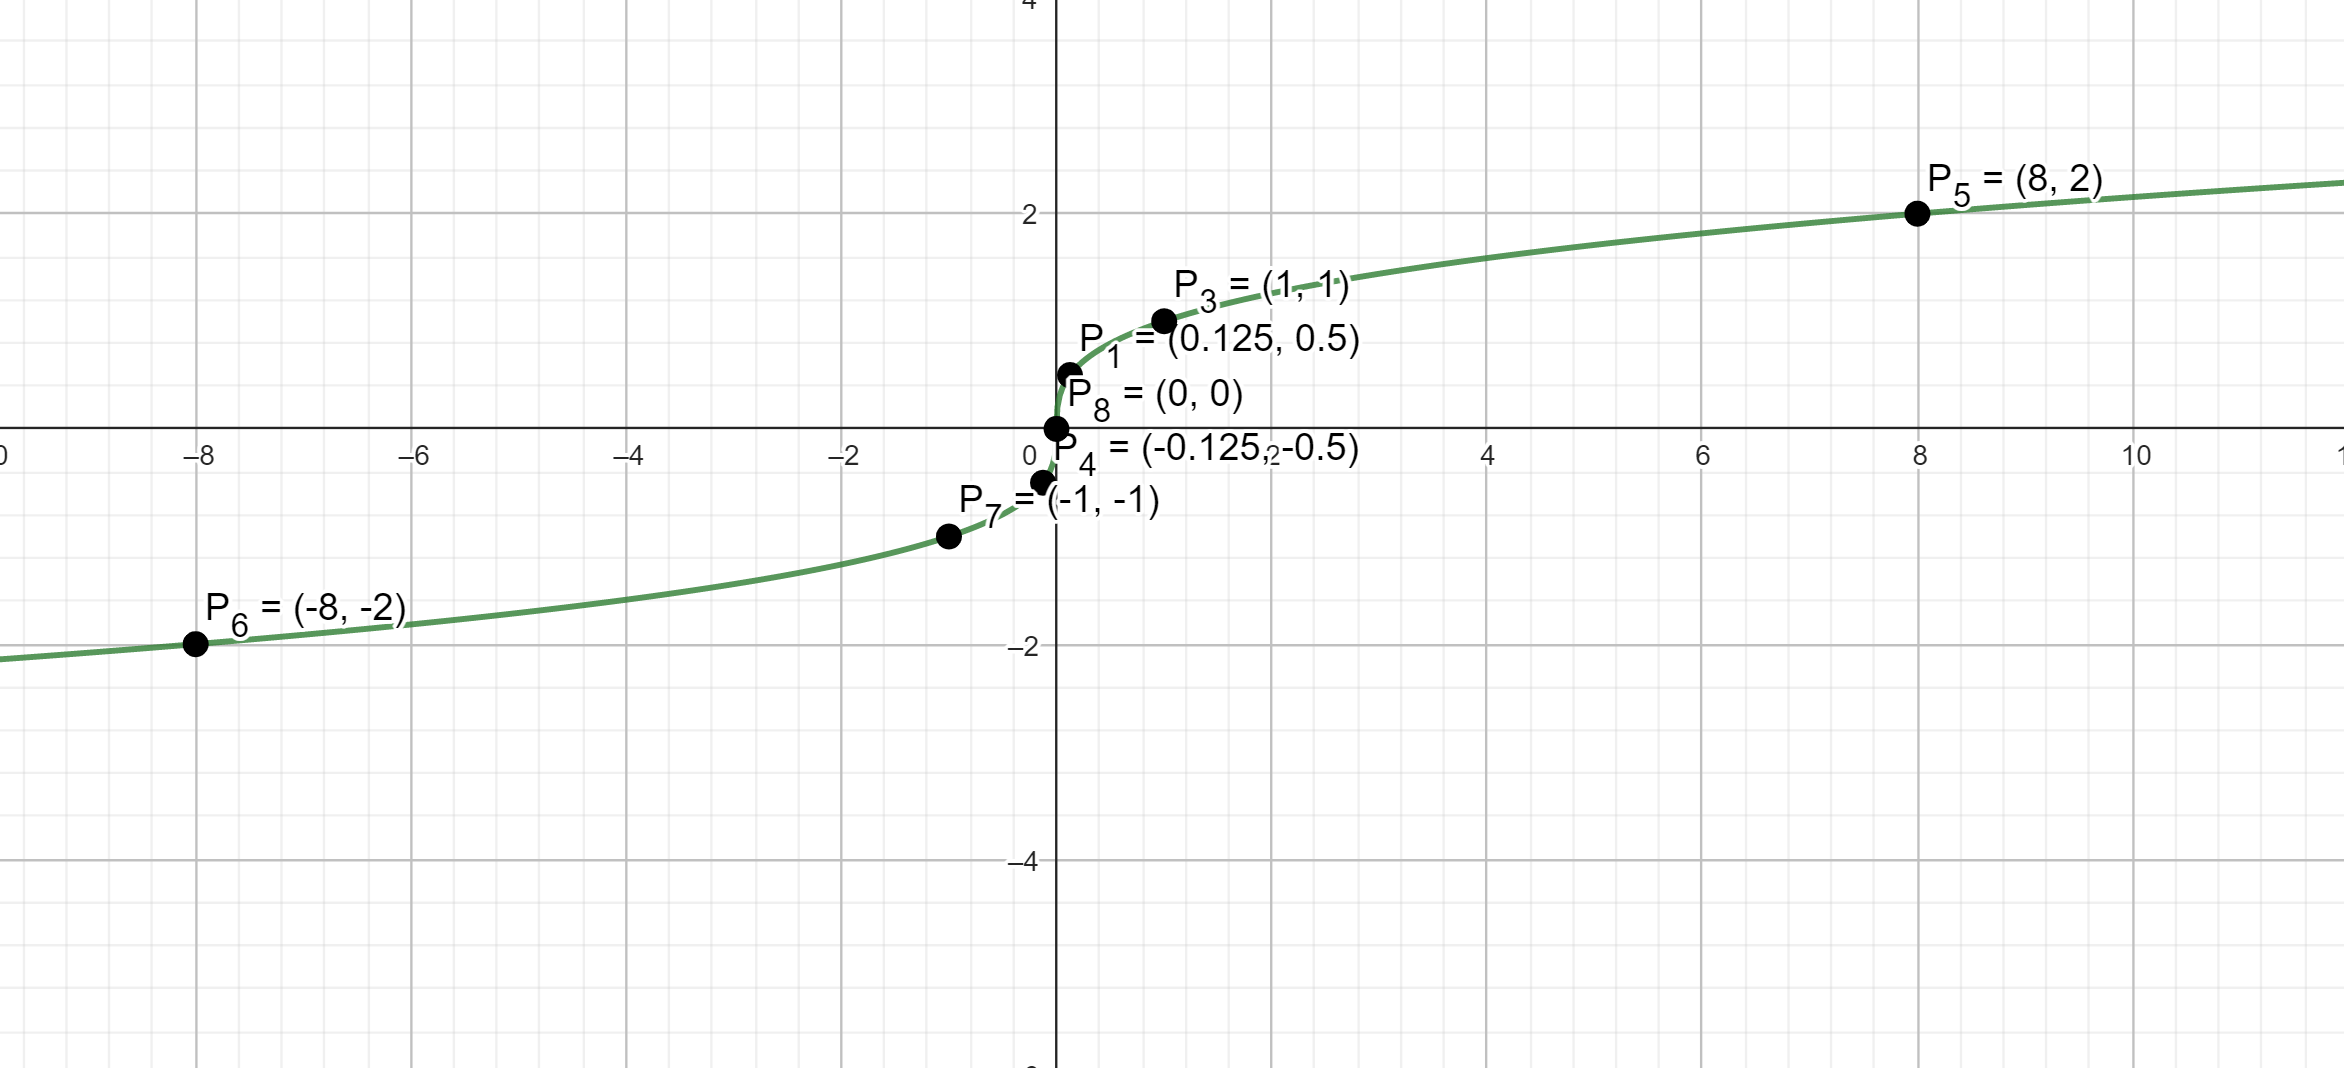
\includegraphics{graficaboletin.png}}
\end{figure}

La función $x_{n + 1} = \sqrt{3x_n}$ es una función raíz cúbica con un dominio en $(-\infty , \infty)$. Además, su imagen existe en todo $\mathbb{R}$ debido a que su crecimiento es continuo. Al analizar las posiciones de los puntos dados, se puede observar que (0, f(0)) corta ambos ejes y que el resto de los puntos solo cortan en la función $f(x)$. Además, estos puntos son equidistantes entre sí.

    \subsection{Monotonía, Cotas y Convergencia}

Sea $(x_n){n \in \mathbb{N}}$ una sucesión real que satisface la ecuación en diferencias $x{n+1} = \sqrt{3}x_n$ con término inicial $x_1 = \frac{1}{8}$. Al calcular algunos términos sucesivos, se puede observar que la sucesión está creciendo en magnitud, lo que indica que es una sucesión creciente con cota superior en $x = 1$.

Para determinar la convergencia de la función, se puede utilizar el criterio de la sucesión: si una sucesión ($x_{n}$) converge a un límite $L$, entonces la función $f(x)$ es convergente en $L$ si y solo si $f(x_{n})$ converge a $f(L)$. En este caso, se puede concluir que $f(x)$ converge a $f(1)$.

\begin{equation}
    x_{n+1} = \sqrt{3}x_n \\
    x_2 = \sqrt[3]{x_1} = \sqrt[3]{\frac{1}{8}} = \sqrt[3]{\frac{1}{2}} \\
    x_3 = \sqrt[3]{x_2} = \sqrt[3]{\sqrt{\frac{1}{2}}} = \sqrt[3]{\frac{1}{\sqrt[3]{2}}} \\
    x_4 = \sqrt[3]{x_3} = \sqrt[3]{\sqrt{\frac{9}{8}}} = \sqrt[3]{\frac{27}{8}}
\end{equation}

La sucesión $(x_n)_{n \in \mathbb{N}}$ es una sucesión creciente con cota superior en $x = 1$. La función $f(x)$ converge a $f(1)$ según el criterio de la sucesión.
b)Sea $(x_n){n \in \mathbb{N}}$ una sucesión real que satisface la ecuación en diferencias $x{n+1} = \sqrt{3}x_n$. Analicemos el comportamiento de la sucesión con término inicial $x_1 = 8$.

Calculamos algunos términos sucesivos:

$x_2 = (x_1)^{1/3} = 8^{1/3} = 2$

$x_3 = (x_2)^{1/3} = 2^{1/3} = 2^{1/3}$

$x_4 = (x_3)^{1/3} = (2^{1/3})^{1/3} \approx 1.08$

Podemos observar que los términos sucesivos $x_2$, $x_3$, $x_4$, etc. están decreciendo en magnitud, por lo que la sucesión es decreciente.

Debido a que nunca se llega a superar el punto, tiene cota inferior en $x = 1$.

Para determinar si una función es convergente, se puede utilizar diversos criterios matemáticos. Criterio de la sucesión: Si una sucesión $(x_n)$ converge a un límite $L$, entonces la función $f(x)$ es convergente en $L$ si y solo si $f(x_n)$ converge a $f(L)$.

En este caso, $f(x)$ converge a $f(1)$.
c)Sea $(x_n){n \in \mathbb{N}}$ una sucesión real que satisface la ecuación en diferencias $x{n+1} = \sqrt{3x_n}$. Analicemos el comportamiento de la sucesión con término inicial $x_1 = 1$.

Calculamos algunos términos sucesivos:
\begin{align*}
x_2 &= (x_1)^{\frac{1}{3}} = 1^{\frac{1}{3}} = 1 \
x_3 &= (x_2)^{\frac{1}{3}} = 1^{\frac{1}{3}} = 1 \
x_4 &= (x_3)^{\frac{1}{3}} = 1^{\frac{1}{3}} = 1
\end{align*}
Podemos observar que los términos sucesivos $x_2, x_3, x_4,$ etc. no están decreciendo ni creciendo en magnitud, por lo que la sucesión es constante. No tiene cotas.

Para determinar si una función es convergente, se puede utilizar diversos criterios matemáticos.

Criterio de la sucesión: Si una sucesión $(x_n)$ converge a un límite $L$, entonces la función $f(x)$ es convergente en $L$ si y solo si $f(x_n)$ converge a $f(L)$.

En este caso, $f(x)$ converge a $f(L)= 1$.

d)\begin{equation}
\text{Sea } (x_n){n \in \mathbb{N}} \text{ una sucesión real que satisface la ecuación en diferencias } x{n + 1} = \sqrt{3}x_n \text{. Analicemos el comportamiento de la sucesión con término inicial } x_1 = -\frac{1}{8}.
\end{equation}

\begin{equation}
\text{Calculamos algunos términos sucesivos: }
\end{equation}

\begin{equation}
x_2 = (x_1)^{\frac{1}{3}} = (-\frac{1}{8})^{\frac{1}{3}} = -\frac{1}{2}
\end{equation}

\begin{equation}
x_3 = (x_2)^{\frac{1}{3}} = (-\frac{1}{2})^{\frac{1}{3}} = -\frac{1}{2^{\frac{1}{3}}}
\end{equation}

\begin{equation}
x_4 = (x_3)^{\frac{1}{3}} = \left[-\frac{1}{2^{\frac{1}{3}}}\right]^{\frac{1}{3}} \approx -0.92
\end{equation}

\begin{equation}
\text{Podemos observar que los términos sucesivos } x_2, x_3, x_4, \text{ etc. no están decreciendo en valor absoluto, por otra parte, al ser un valor negativo, } x_1 > x_2 \text{ por lo que la sucesión es decreciente.}
\end{equation}

\begin{equation}
\text{Tiene cota inferior en } f(x) = -1.
\end{equation}

\begin{equation}
\text{Para determinar si una función es convergente, se puede utilizar diversos criterios matemáticos.}
\end{equation}

\begin{equation}
\text{Criterio de la sucesión: Si una sucesión } (x_n) \text{ converge a un límite } L, \text{ entonces la función } f(x) \text{ es convergente en } L \text{ si y solo si } f(x_n) \text{ converge a } f(L).
\end{equation}

\begin{equation}
\text{En este caso, } x_{n} \text{ converge a } f(L)= -1.
\end{equation}
c)Sea $(x_n){n \in \mathbb{N}}$ una sucesión real que satisface la ecuación en diferencias $x{n+1} = \sqrt{3x_n}$. Analicemos el comportamiento de la sucesión con término inicial $x_1 = 1$.

Calculamos algunos términos sucesivos:
\begin{align*}
x_2 &= (x_1)^{\frac{1}{3}} = 1^{\frac{1}{3}} = 1 \
x_3 &= (x_2)^{\frac{1}{3}} = 1^{\frac{1}{3}} = 1 \
x_4 &= (x_3)^{\frac{1}{3}} = 1^{\frac{1}{3}} = 1
\end{align*}
Podemos observar que los términos sucesivos $x_2, x_3, x_4,$ etc. no están decreciendo ni creciendo en magnitud, por lo que la sucesión es constante. No tiene cotas.

Para determinar si una función es convergente, se puede utilizar diversos criterios matemáticos.

Criterio de la sucesión: Si una sucesión $(x_n)$ converge a un límite $L$, entonces la función $f(x)$ es convergente en $L$ si y solo si $f(x_n)$ converge a $f(L)$.

En este caso, $f(x)$ converge a si mismo $f(L)= 1$.

e)Sea $(x_n){n \in \mathbb{N}}$ una sucesión real que satisface la ecuación en diferencias $x{n+1} = \sqrt{3}x_n$. Analicemos el comportamiento de la sucesión con término inicial $x_1 = -8$.

Calculamos algunos términos sucesivos:

$x_2 = (x_1)^{1/3} = -8^{1/3} = -2$

$x_3 = (x_2)^{1/3} = 2^{1/3} = (-2)^{1/3}$

$x_4 = (x_3)^{1/3} = ((-2)^{1/3})^{1/3} \approx -1.08$

Podemos observar que los términos sucesivos $x_2$, $x_3$, $x_4$, etc. están decreciendo en magnitud, pero en valor real crece pro lo que la sucesion es creciente.

Debido a que nunca se llega a superar el punto, tiene cota superior en $x = -1$.

Para determinar si una función es convergente, se puede utilizar diversos criterios matemáticos. Criterio de la sucesión: Si una sucesión $(x_n)$ converge a un límite $L$, entonces la función $f(x)$ es convergente en $L$ si y solo si $f(x_n)$ converge a $f(L)$.

En este caso, $f(x)$ converge a $f(-1)$.

f)Sea $(x_n){n \in \mathbb{N}}$ una sucesión real que satisface la ecuación en diferencias $x{n+1} = \sqrt{3x_n}$. Analicemos el comportamiento de la sucesión con término inicial $x_1 = -1$.

Calculamos algunos términos sucesivos:
\begin{align*}
x_2 &= (x_1)^{\frac{1}{3}} = 1^{\frac{1}{3}} = -1 \
x_3 &= (x_2)^{\frac{1}{3}} = 1^{\frac{1}{3}} = -1 \
x_4 &= (x_3)^{\frac{1}{3}} = 1^{\frac{1}{3}} = -1
\end{align*}
Podemos observar que los términos sucesivos $x_2, x_3, x_4,$ etc. no están decreciendo ni creciendo en magnitud, por lo que la sucesión es constante. No tiene cotas.

Para determinar si una función es convergente, se puede utilizar diversos criterios matemáticos.

Criterio de la sucesión: Si una sucesión $(x_n)$ converge a un límite $L$, entonces la función $f(x)$ es convergente en $L$ si y solo si $f(x_n)$ converge a $f(L)$.

En este caso, $f(x)$ converge a si mismo $f(L)= -1$.

h)Sea $(x_n){n \in \mathbb{N}}$ una sucesión real que satisface la ecuación en diferencias $x{n+1} = \sqrt{3x_n}$. Analicemos el comportamiento de la sucesión con término inicial $x_1 = 0$.

Calculamos algunos términos sucesivos:
\begin{align*}
x_2 &= (x_1)^{\frac{1}{3}} = 1^{\frac{1}{3}} = 0 \
x_3 &= (x_2)^{\frac{1}{3}} = 1^{\frac{1}{3}} = 0 \
x_4 &= (x_3)^{\frac{1}{3}} = 1^{\frac{1}{3}} = 0
\end{align*}
Podemos observar que los términos sucesivos $x_2, x_3, x_4,$ etc. no están decreciendo ni creciendo en magnitud, por lo que la sucesión es constante. No tiene cotas.

Para determinar si una función es convergente, se puede utilizar diversos criterios matemáticos.

Criterio de la sucesión: Si una sucesión $(x_n)$ converge a un límite $L$, entonces la función $f(x)$ es convergente en $L$ si y solo si $f(x_n)$ converge a $f(L)$.

En este caso, $f(x)$ converge a $f(L)= 0$.

    \subsection{Clasificación del Límite}

Conociendo los valores de los límites de cada punto, pasamos a hacer la clasificación de estos; podemos llegar a una conclusión del tipo de límite si:
        -El límite de la sucesión $\liminf[n]{\sqrt[3]{x_{n+1}}} = L \implies L = \sqrt[3]{L} \implies L = 0 $
        -Si x>0, es convergente al lim L = 0
        -Si x=, es constante y su valor es 0 siempre
        -Si x<0 la sucesión no tiene límite ya que no está definida en valores < 0 debido a la función anterior.
        Solución:
        convergentes: a b c
        constantes: g
        divergentes: d e f


\section{Ejercicio 3}

\text{Analiza la convergencia o divergencia de la siguiente serie de números reales en función al valor del parámetro x $\in R$ :
$\sum \infty$ [$x^n/n$]
n=1}

\subsection{Solución problema 3}

Se puede analizar la convergencia del sumatorio de la función mediante el criterio de la raiz:
$L = \liminf[n]{\sqrt[n]{\frac{x_{n}}{n}}} = \liminf{\sqrt[n]{x*\frac{1}{n}}} = x*0 = 0$

Ya que el limite en el infinito de la función radicando tiende a 0 en el infinito.
Analizando en conjunto con el criterio de la raiz, llegamos a la conclusión de que L = 0 y que L < 1 
por lo que la serie es convergente absoluta.

\end{document}
